\section{Die Landkreise und Regierungsbezirke sortiert nach dem Gemeindeschlüssel}
In \autoref{fig:distribution_AdmUnitId} lässt sich an der Farbe der Landkreise/Regierungsbezirke grob erkennen, in welcher Reihenfolge diese behandelt werden, wenn sie in der Reihenfolge ihrer Gemeindeschlüssel benutzt werden.
\begin{figure}[H]
    \centering
    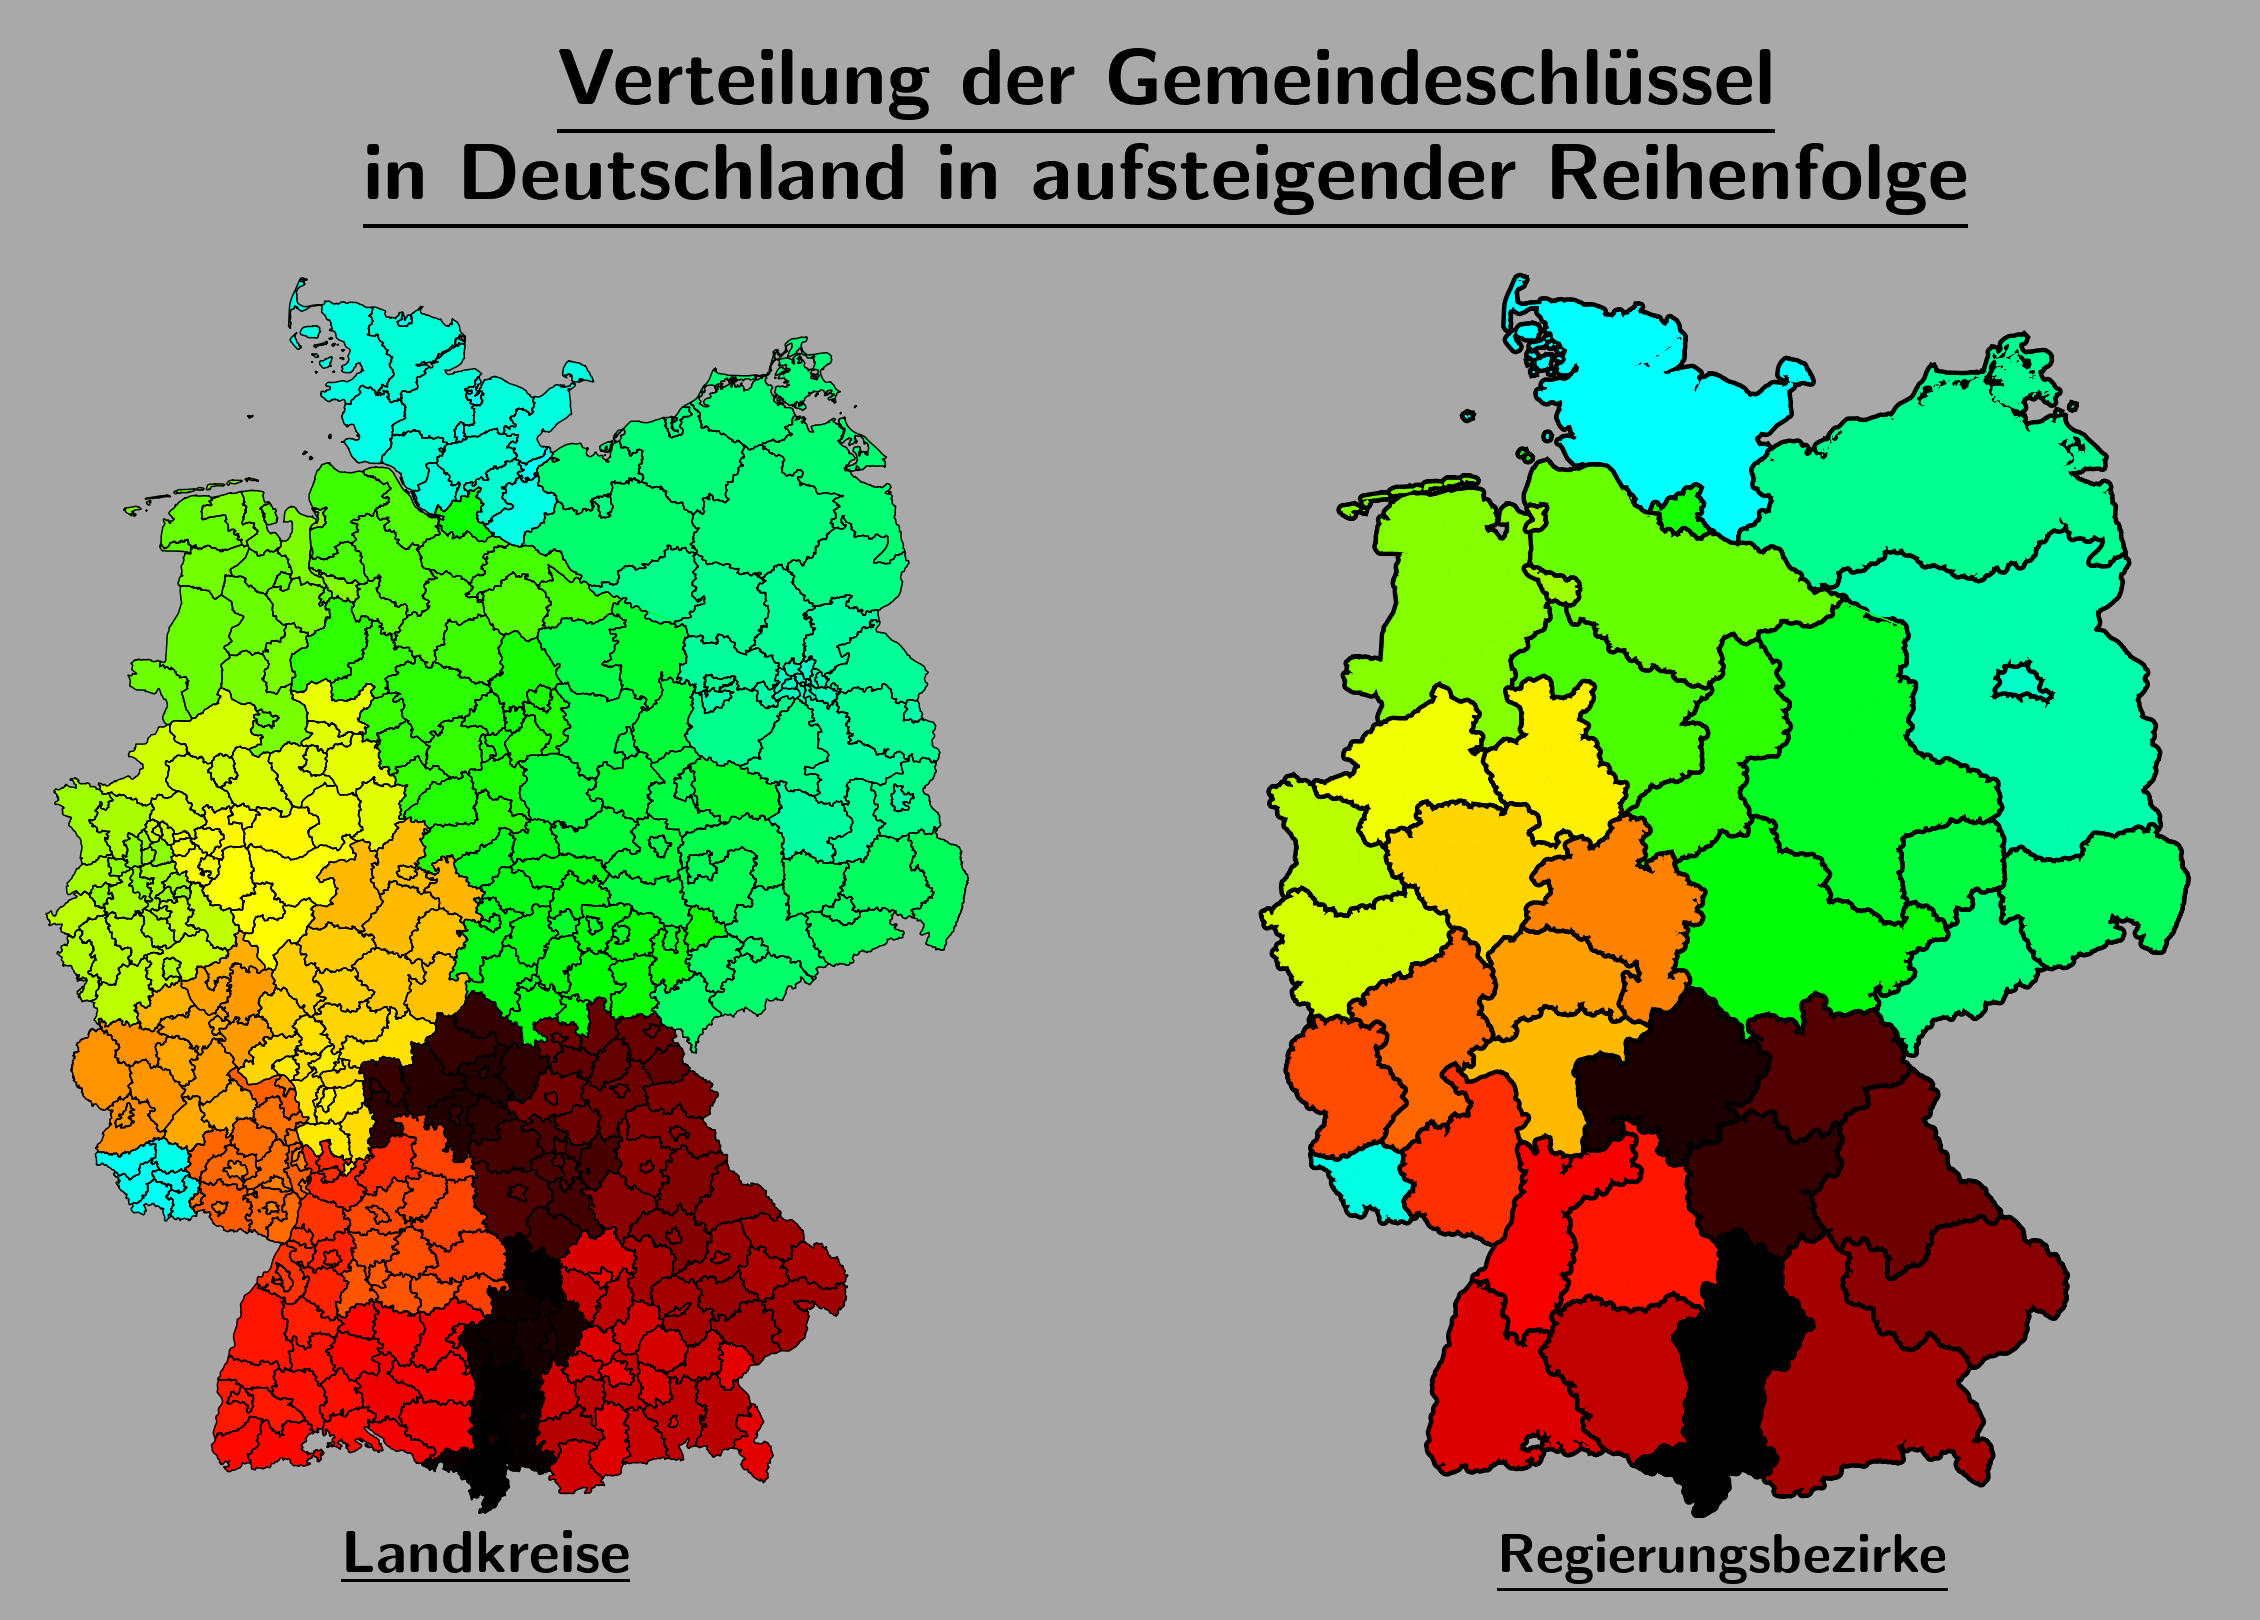
\includegraphics[width = 0.95\textwidth]{figures/Ergebnisse/districts_and_counties_by_AdmUnitID.png}
    \caption{Die Landkreise und Regierungsbezirke eingefärbt nach der lexikographischen Größe ihres Gemeindeschlüssels. Bei blau beginnend werden den nach ihrem Gemeindeschlüssel sortierten Landkreise die Farbfolge des Regenbogens zugeteilt.}
    \label{fig:distribution_AdmUnitId}
\end{figure}